\chapter{Results Obtained}
\label{cha:results obtained}
\section{Test Models}
\label{sec:test models}
This chapter shows the performances of the algorithms previously discussed, focusing on a standard version developed on Edge Impulse\cite{edgeimpulse_kws_example}, 2 d-vector versions, one emulating an existing solution\cite{dvector_extractor_TinySV} (d-vector extractor size 256) and another solution with size 128, that could be adapted to the system, to reduce the required dimension in the dataset storage, and 5 distilled models (1 from 128 version and 4 from 256 one). The reason, why various versions of 256 d-vector size were generated, is due to not fitting. To be deployed on Syntiant after distillation, the models have to be quantized in 4-int weights. Knowing that the model can host at most 589.000 4-int parameters, the solution for 128's version is straightforward in converting to a consistent dense model; in contrast, the 256's version is harder to adapt to these tiny dimensions. To determine if a model can be hosted in a Syntiant NDP101, knowing that the dense layers are 3 intermediate and one output. The formula to compute the model's size of a dense neural network is the following:
\begin{equation*}
    model\_size=\sum_{i=1}^{N}((in\_size_i+1)*out\_size_i)\,\,\,\,\,condition:\,\,model\_size<294.500\,bytes
\end{equation*} 
Instead, to compute the one of a convolutional neural network should be used this one because of multidimensionality, considering a general filter shape like (width, height, channels):
\begin{equation*}
    model\_size=\sum_{i=1}^{N}((in\_channels*f\_width*f\_height+1)*out\_channels)
\end{equation*}
Following, there is a table summarizing which model will be deployable on Syntiant:
\begin{table}[!h]
    \label{tabel:model sizes}
\centering
    \begin{tabular}{|c|c|c|c|c|c|c|c|c|}
        \hline
        Model Name & KWS & SV128 & SV256 & SVD128 & SVDU256 & SVD192 & SVD240 & SVD2256\\
        \hline
        Type & Dense & Conv & Conv & Dense & Dense & Dense & Dense & Dense\\
        Origin & - & - &  - & SV128 & SV256 & SV256 & SV256 & SV256\\
        Input & 1600 & (40x40x1) & (40x40x1) & 1600 & 1600 & 1600 & 1600 & 1600\\
        Layer 1 & 256 & (13x13x8) & (13x13x8) & 256 & 256 & 192 & 240 & 256\\
        Layer 2 & 256 & (6x6x16) & (6x6x16) & 256 & 256 & 192 & 240 & 256\\
        Layer 3 & 256 & (3x3x32) & (3x3x32) & 256 & 128 & 192 & 240 & 256\\
        Layer 4 & - & (2x2x64) & - & - & - & - & - & -\\
        Layer Out & 2 & 128 & 256 & 128 & 256 & 256 & 256 & 256\\
        Total (KB) & 2117 & 383,6 & 95,2 & 2243,5 & 2115,5 & 1683,25 & 2193,8 & 2372\\
        Deployable & YES & NO & NO & YES & YES & YES & YES & NO\\
        \hline
    \end{tabular}
    \caption{Model Dimension Details}
\end{table}
Note that the width and height of the convolution formula are used for filter size, instead, in the table above, there are the input and the output of the steps. The filter always is (3x3xchannels), with channels instead of the ones present in the datasheet. The condition for a model to be deployable in float configuration, before quantization, is that it should be smaller than 2300 KB, and it should be a dense model. The choice of the distillation models having as father 256-size version are respectively:\newline
• U256 - consisting of an unbalanced distribution of neurons, having a layer downscaling to 218 from the standard of 256 to fit inside the Flash memory\newline
• 192 - considering that model neurons should be typically a power of two, considering 128 neurons in all layers too restrictive to mimic the father's behavior, it was chosen a general multiple of two with a reasonable value that fits inside the device\newline
• 240 - it was the optimal multiple of 2 that could fit inside the device, having all the intermediate layers with equal neurons and the output of 256\newline
• 256 - this model does not fit, but was used to compare the behavior with another model with 256 neurons in intermediate layers and 128 d-vector as output\newline\newline
If the KWS performs a classification, having a direct output, SV performs a cosine similarity with d-vectors saved as references. This is done to view various perspectives of which version of the model is better considering performance and size perspectives. The methodologies of d-vector comparison used are 3:\newline
1. Best matching - it takes the highest cosine similarity value when comparing each reference vector with the vector obtained as a result of the Speaker Verification model. It requires that all the reference vectors are saved in memory\newline
2. Mean d-vector - it is computed the mean d-vector performing the average among each d-vector and then using this obtained vector is performed a cosine similarity and the score obtained will be the result. In this case, it should be saved only the mean d-vector saving more space\newline
3. Geometrical Median - it is an optimized version of mean computation. It implements Weiszfeld's algorithm\cite{weiszfeldsalgorithm}, which is an iterative method to compute the geometric median of a set of points present in an Euclidean space. It is more computationally expensive because at first requires a mean computation. Then, some weights computation to minimize the distance between the points, to obtain an optimized d-vector. The algorithm is the one below:\newline
\begin{algorithm}[H]
\caption{Geometric Median via Weiszfeld’s Algorithm}
\KwIn{Set of $n$ vectors $\{\mathbf{x}_1, \mathbf{x}_2, \dots, \mathbf{x}_n\} \subset \mathbb{R}^d$}
\KwOut{Approximate geometric median $\mathbf{z} \in \mathbb{R}^d$}
\nl \textbf{Initialize:} Set initial estimate $\mathbf{z}^{(0)} \gets \frac{1}{n} \sum_{i=1}^n \mathbf{x}_i$\;
\nl \For{$t \gets 0$ \KwTo $T_{\max}$}{
    \nl Set $w_{\text{sum}} \gets 0$\;
    \nl Set $\mathbf{z}_{\text{new}} \gets \mathbf{0} \in \mathbb{R}^d$\;
    \nl \For{$i \gets 1$ \KwTo $n$}{
        \nl Compute $d_i \gets \|\mathbf{x}_i - \mathbf{z}^{(t)}\|$\;
        \nl \If{$d_i < \varepsilon$}{
            \nl \textbf{continue} \tcp*{Skip or optionally snap to $\mathbf{x}_i$}
        }
        \nl Compute weight $w_i \gets \frac{1}{d_i}$\;
        \nl Update weighted sum: $\mathbf{z}_{\text{new}} \gets \mathbf{z}_{\text{new}} + w_i \cdot \mathbf{x}_i$\;
        \nl Update weight sum: $w_{\text{sum}} \gets w_{\text{sum}} + w_i$\;
    }
    \nl \If{$w_{\text{sum}} = 0$}{
        \nl \textbf{break} \tcp*{All points are too close; cannot proceed}
    }
    \nl Normalize: $\mathbf{z}^{(t+1)} \gets \frac{\mathbf{z}_{\text{new}}}{w_{\text{sum}}}$\;
    \nl \If{$\|\mathbf{z}^{(t+1)} - \mathbf{z}^{(t)}\| < \varepsilon$}{
        \nl \textbf{break} \tcp*{Converged}
    }
}
\KwRet{$\mathbf{z}^{(t+1)}$}
\end{algorithm}
To each of these method the number of reference d-vector used was 1, 8, 16 and 64; it is relevant to note that 1 result should be the same in all 3 modes. This references' dataset with size of 64 KB on a SRAM of 128 KB. The components of d-vector changes, because the default size-type model is float, but Syntiant quantizes it in 4-int weights, but the performances could not be verified because of the NDA, so were used in float format.\newline\newline
Because of being a TinySV with an objective of using internal memory for dataset, too, it is important to consider the size, allowing evaluation on how many words and consequently how many users can be inserted in the logic depending on the usage. They are inverse proportionate having $num\,of\,users\cdot words\,categories=total\,num\,fitable\,on\,Syntiant$ and the total number on Syntiant vary according to the method used and the number of references. In the case of bestmatching technique, having an higher number of references, leads in having less words, because a word representation will require more space.\newline
\begin{table}[!h]
    \label{table:word sizes}
    \centering
    \renewcommand{\arraystretch}{1.2}
    \begin{tabular}{|c|cccccc|}
        \hline
        \textbf{Type} & \multicolumn{6}{c|}{\textbf{D-vector = 128}} \\
        \hline
        \textbf{Aggregation} & \multicolumn{4}{c}{\textbf{Best}} & \textbf{Mean} & \textbf{Geom\_Median} \\
        \hline
        \textbf{N° Refs} & \textbf{1} & \textbf{8} & \textbf{16} & \textbf{64} & \textbf{All} & \textbf{All} \\
        \hline 
        \textbf{Size of Word (B)} & 512 & 4096 & 8192 & 32768 & 512 & 512 \\
        \textbf{Quant (B)}        & 64 & 512 & 1024 & 4096 & 64 & 64 \\
        \textbf{Words Float}      & 128 & 16 & 8 & 2 & 128 & 128 \\
        \textbf{Words 4-int}      & 1024 & 128 & 64 & 16 & 1024 & 1024 \\
        \hline
        \textbf{Type} & \multicolumn{6}{c|}{\textbf{D-vector = 256}} \\
        \hline
        \textbf{Aggregation} & \multicolumn{4}{c}{\textbf{Best}} & \textbf{Mean} & \textbf{Geom\_Median} \\
        \hline
        \textbf{N° Refs} & \textbf{1} & \textbf{8} & \textbf{16} & \textbf{64} & \textbf{All} & \textbf{All} \\
        \hline 
        \textbf{Size of Word (B)} & 1024 & 8192 & 16384 & 65536 & 1024 & 1024 \\
        \textbf{Quant (B)}        & 128 & 1024 & 2048 & 8192 & 128 & 128 \\
        \textbf{Words Float}      & 64 & 8 & 4 & 1 & 64 & 64 \\
        \textbf{Words 4-int}      & 512 & 64 & 32 & 8 & 512 & 512 \\
        \hline
    \end{tabular}
    \caption{Dataset dimensional configuration based on aggregation type and number of references}
    \label{table:dataset_dimensions}
\end{table}
\section{Testing Dataset and Performance Metrics}
\label{sec:testing dataset and performance metrics}
The various models were tested with a composed dataset containing one second audio samples of my own voice saying a train word (Sheila), other users' voice saying the same word, but different from the ones using during training\cite{librispeech} and some samples of total different words and some that may sound like the chosen word. In the KWS model, the first two cases will output TP and FN, meanwhile the third category will output FP and TN. Instead, for SV models, only the words that were considered TP would be processed, however considering that some reference d-vector had to be chosen randomly, was created an algorithm threshold that in the case the similarity was above 0.99, the sample has to be truncated. Because of this limitation in Convolutional Models, there are fewer samples, because they where eliminated to not ruin the results, instead with distillation is predicted a loss in cosine similarity, because is a trying in mimic the convolution behavior with simple multiplication and addition, so even the reference samples passed in the neural network will not be processed as the same ones.\newline\newline
Quantitative talking, the test dataset is composed by:\newline
• 485 Sheila Owner Samples (registered manual and split in one-second samples using Edge Impulse\cite{syntiant_tutorial_edgeimpulse})\newline
• 2022 Sheila Others Samples (taken by Google Command Dataset\cite{speechcommands} corresponding to Sheila word)\newline
• 474 Similar Sheila Words (taken by Google Command Dataset\cite{speechcommands} not corresponding to Sheila word)\newline
This leads to a total of 2981 samples used for KWS, but for SV to be sure that only true Sheila words were passed were accepted only with a probability of being Sheila higher than 0.8, so the TP samples of KWS which are higher than that value.\newline\newline
Other than size metrics, there are some performance metrics previously introduced in chapter 2 that will be used in the evaluation of each model performance. The threshold on which a value is determined to be or not true depends on EER Threshold, which is the best value in which the FPR and the FNR are as close as possible. On this threshold were computed:\newline
• Accuracy: Rate of results corresponding with expectations over total elements (High better)\newline
• Classification Loss: Rate of results not corresponding with expectations over total elements (Lower better)\newline
• Precision: Rate of true expectations over all samples which result is true (High better)\newline
• Recall: Rate of true results over all samples expected to be true (High better)\newline
• F1 Score: An estimated score to evaluate the performance considering precision and recall (High better)\newline
• EER: Is the highest value among the false acceptance rate and the false rejection rate, even though they should be similar, because the threshold is equal to the ERR point (Low better)\newline
• AUC: Is the area under the curve that in a binary classification that if around 0.5 indicates random guesses, instead higher values represents more deterministic results (High better)\newline
\section{Experiment performances}
\label{sec:experiment performance}
\subsection{KWS}
\label{subsec:kws performance}
Starting with the analysis of the results obtained, the first model to explore will be KWS. The classification it as of know binary, but according to the Syntiant, the maximum trainable keyword spotting words are 64.\cite{description_ndp101}. The computation of the performance like calculation of AUC and ERR were in a range of 0.5 and 1 thresholds. According to the results obtained the threshold is around 0.7 with 90\% of true positive out of 2507, expected true samples, and 90,11\% of true negative out of 474 samples. The model overall performs well with a low Equal Error Rate and a decent AUC value, compensating with good accuracy, optimal precision and good recall. Leading to the following results:\newline
\begin{table}[!h]
\centering
%\caption{KWS Model Evaluation Results}
\label{table:kws_centered}
\small
\begin{tabular}{@{}m{3.8cm}@{\hspace{1em}}m{3.8cm}@{\hspace{1em}}m{3.8cm}@{\hspace{1em}}m{3.8cm}@{}}
\toprule
\multicolumn{1}{c}{\textbf{Configuration}} & \multicolumn{1}{c}{\textbf{Data Analysis}} & \multicolumn{1}{c}{\textbf{Performance}} & \multicolumn{1}{c}{\textbf{Quality}}\\
\midrule

\centering
\textbf{Model:} KWS \\
\textbf{Threshold:} 0.7 \\
\textbf{Total Samples:} 2981 &

\centering
\textbf{Confusion Matrix:} \\
TP: 2259, FN: 248 \\
FP: 48, TN: 426 \\[0.3em]
\textbf{Distribution:} \\
Pos: 2507 (84.1\%) \\
Neg: 474 (15.9\%) &

\centering
\textbf{Classification:} \\
Accuracy: 90.1\% \\
Precision: 97.9\% \\
Recall: 90.1\% \\
F1: 93.9\% &

\centering
\textbf{Quality:} \\
EER: 0.101 \\
AUC: 0.885 \\

\tabularnewline
\bottomrule
\end{tabular}
\end{table}
\subsection{Speaker Classification of CNN Model}
\label{subsec:speaker classification of cnn model}
\begin{figure}[!h]
    \begin{minipage}[b]{0.33\textwidth}
            \centering
            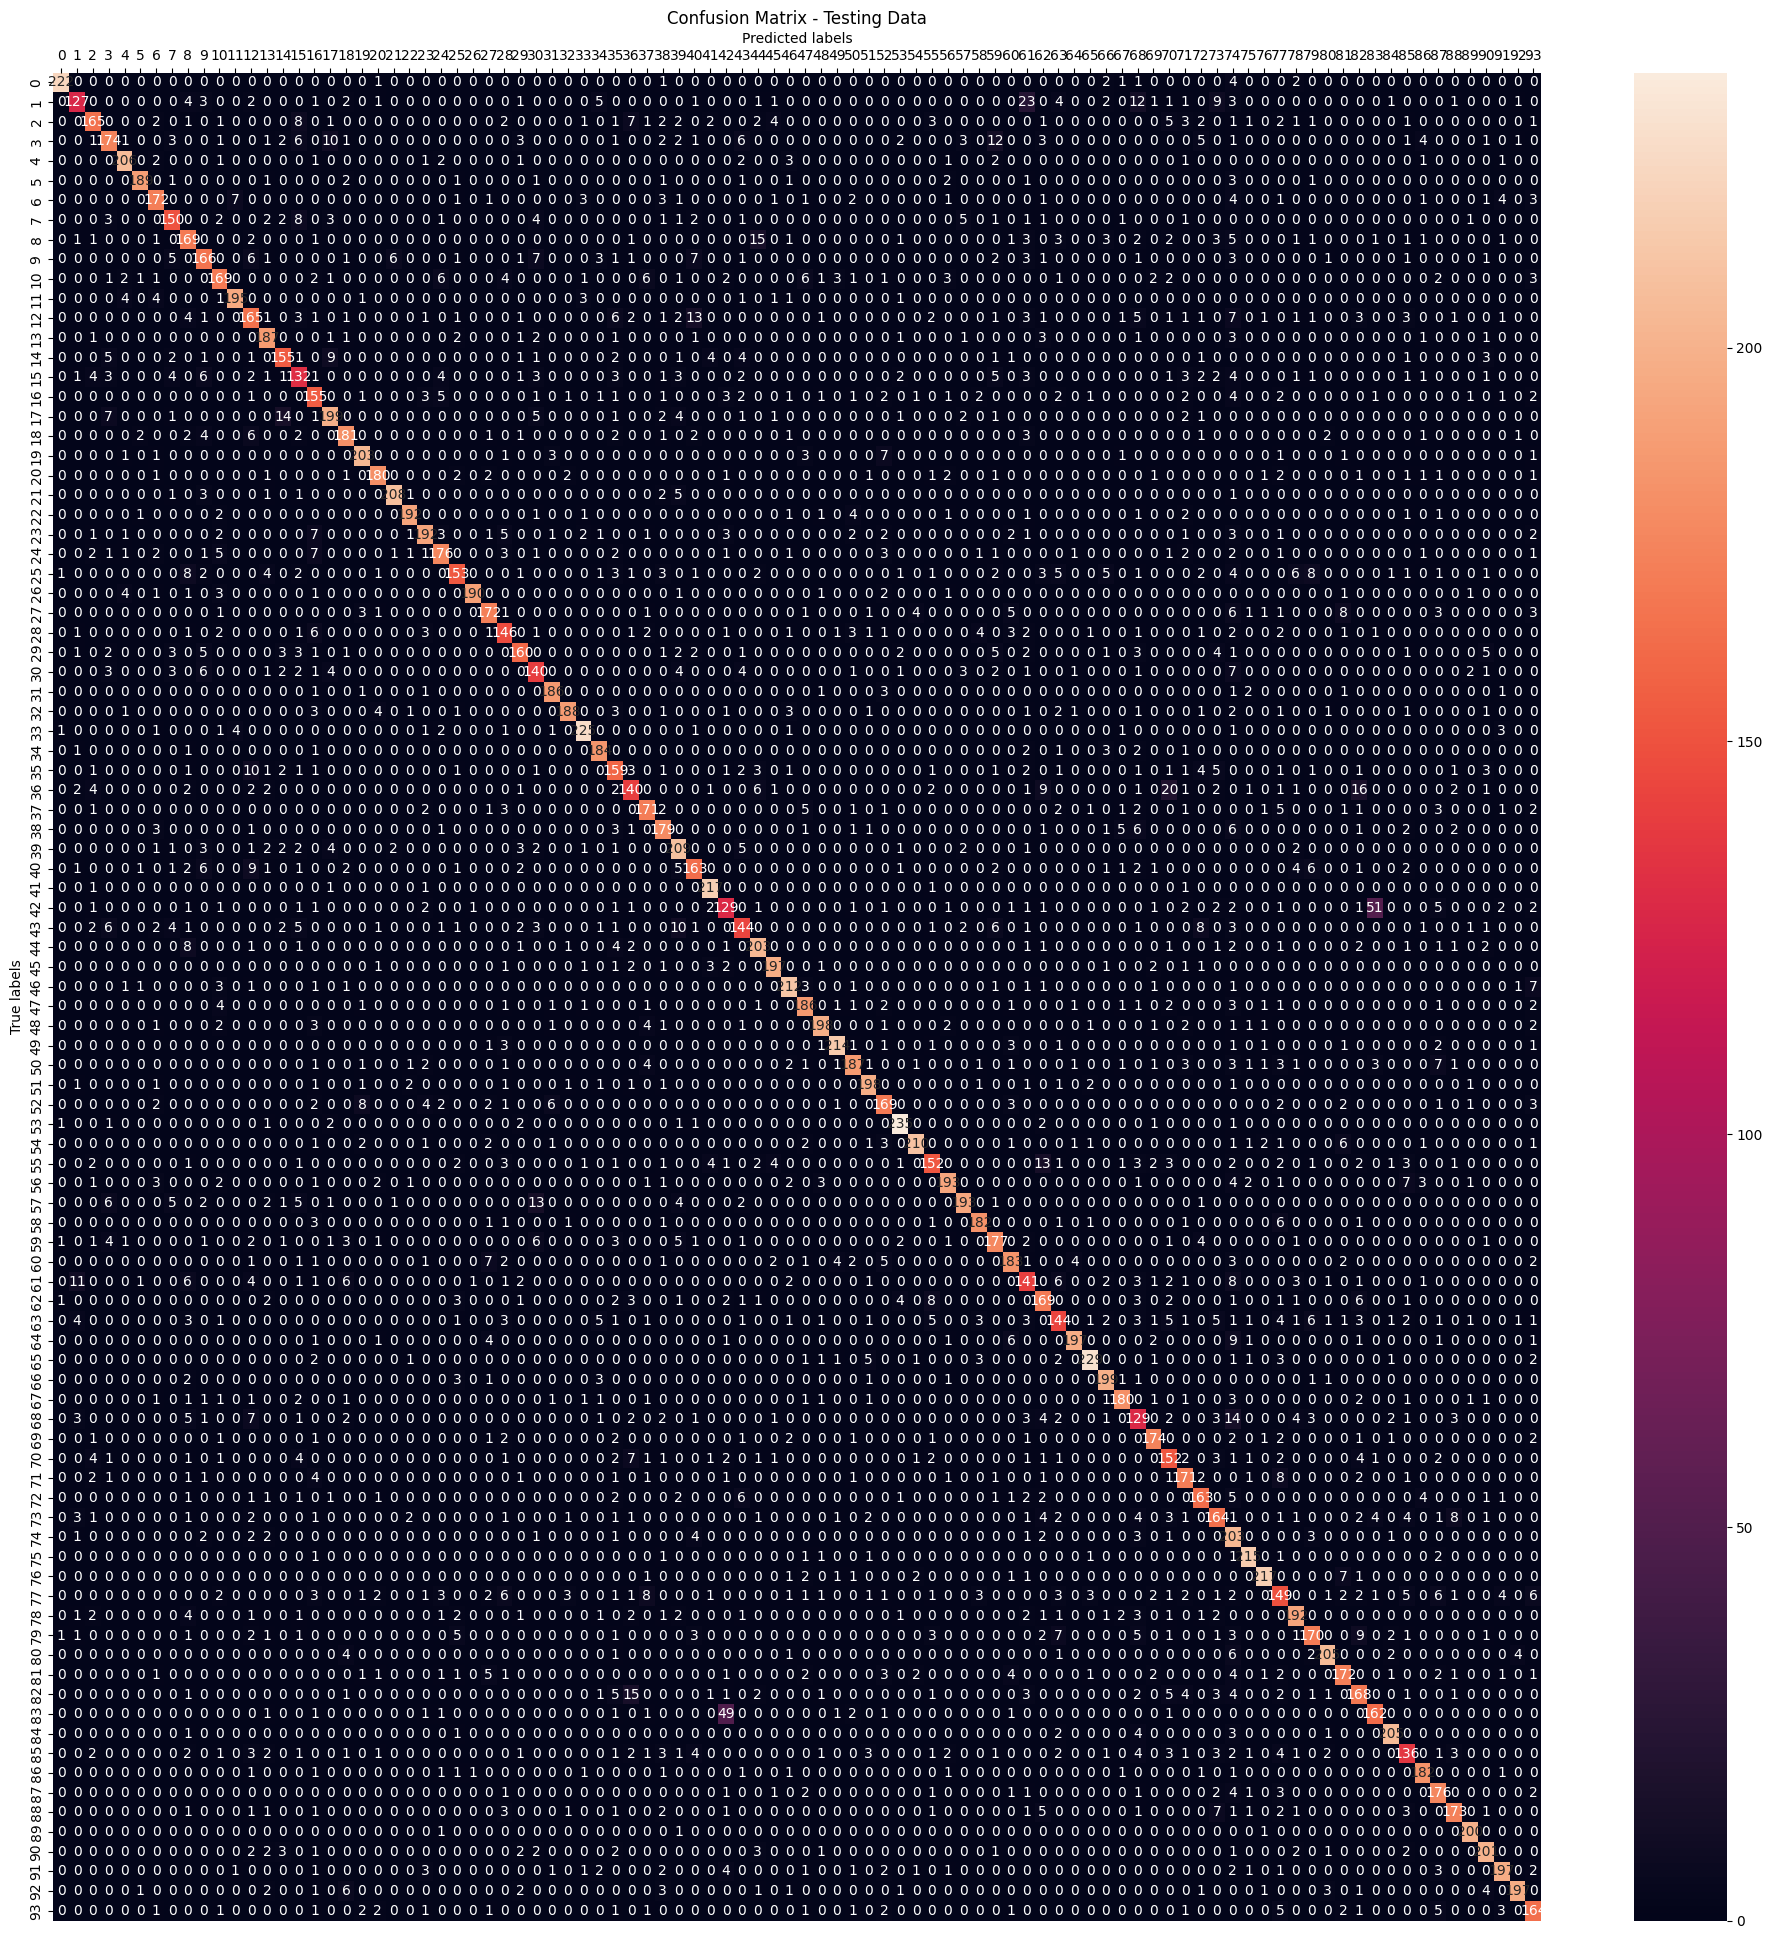
\includegraphics[width=\textwidth]{images/5.01 CCN Confusion Matrix.png}
            \caption{Confusion Matrix}
            \label{fig:confusion matrix}
    \end{minipage}
    \hfill
    \begin{minipage}[b]{0.67\textwidth}
            \centering
            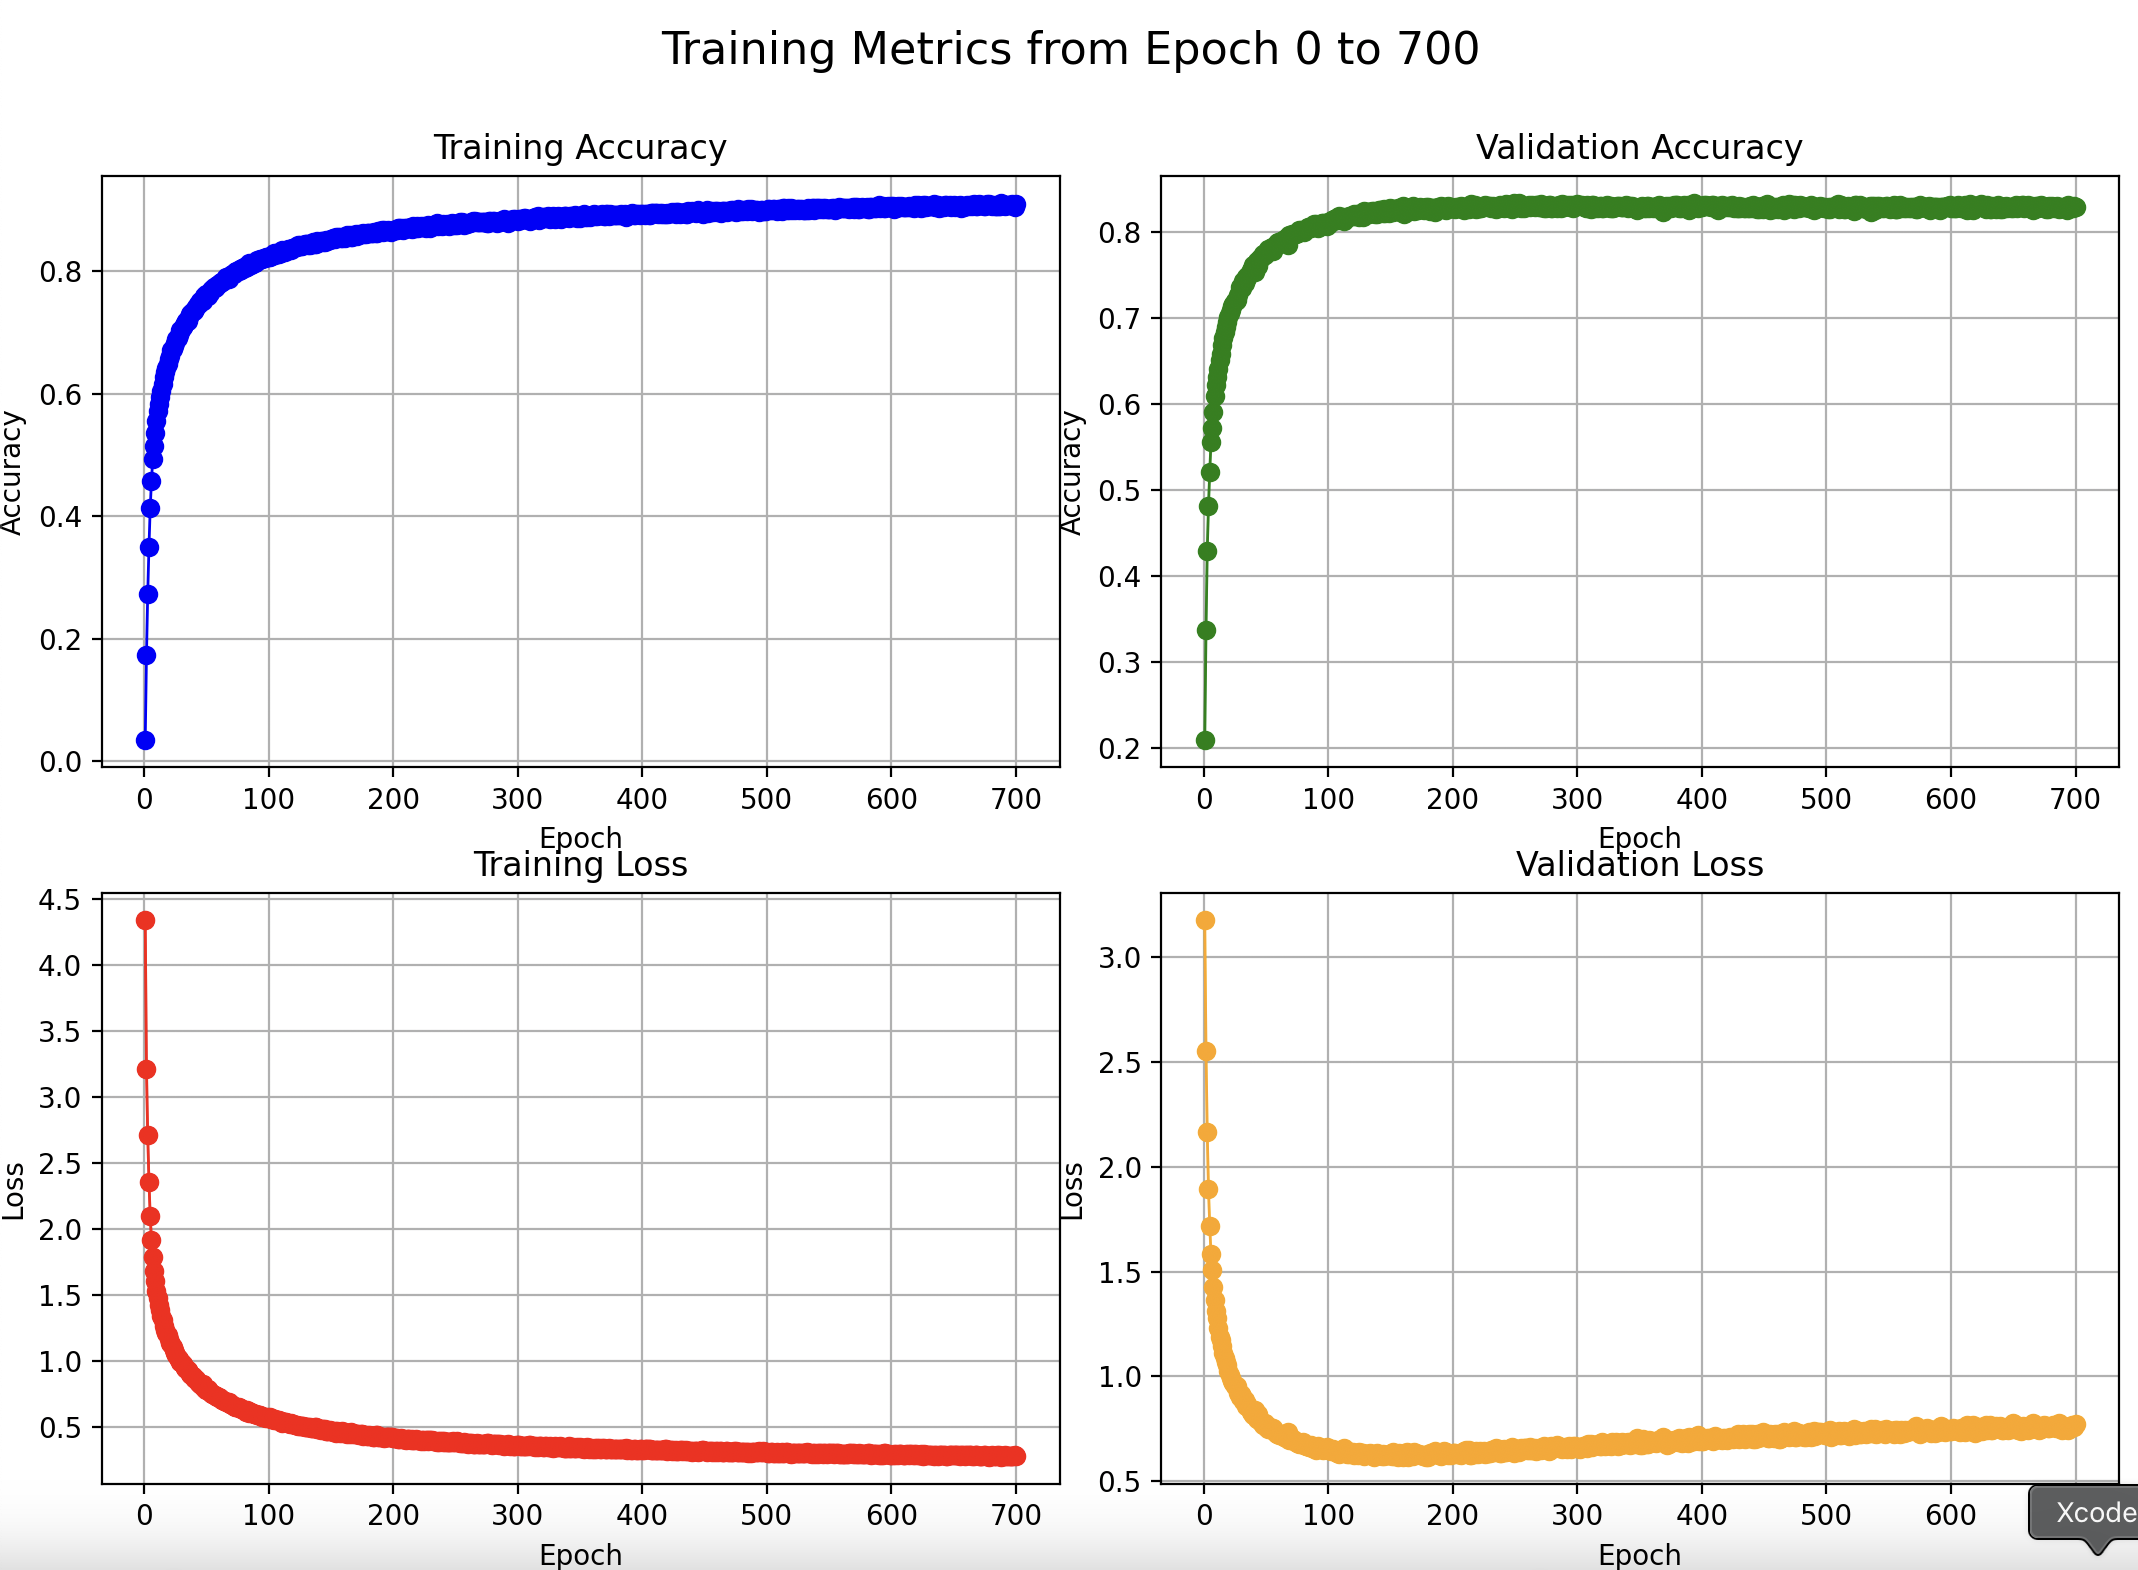
\includegraphics[width=0.8\textwidth]{images/5.02 CNN Training Details.png}
            \caption{CNN Training Details}
            \label{fig:cnn training details}
    \end{minipage}
\end{figure}
If KWS is only a single model that can be optimized and handled during time, SV purpose is to be a one-training model. Because of this, is really important to determine the best configuration possible for a deployment. As start, it is interesting to analyze the confusion matrix obtained by the classification of the original convolutional model before the truncation. 
The training was performed with 700 epochs using as accuracy parameters the correspondence of the samples results with the expectations, instead the Loss was computed with two callbacks:\newline
1. ReduceLROnPlateau: in case the training loss doesn't improve (decreases), the learning rate is reduce by a factor. In this case, was applied a patience of 10 and a factor of 0.5.\newline
2. EarlyStopping: in case the training loss doesn't improve, the training is stopped early. In this case, it was set a patience of 20, but most importantly this allows to restore the best weights from the epoch with the lowest training loss, to get the values, before the model overfits. The overfitting is when a model learns data too well, including the outliers or random fluctuations, performing poorly with unseen data.
As result is obtained an accuracy around 83\% of accuracy, meanwhile there is a 61\% of loss. The reason why there is still a high loss is because the presence of only an intermediate layer, other than the output one, dense layer's talking. This leads to less precision because mapping out 94 users may be difficult in a classification, however all of this was done only to give the d-vector, to see how accurate it may be using a classification.
\subsection{SV Convolutional Models}
\label{subsec:sv convolutional models}
The two d-vector extractors obtained truncating the classification part are the one with 128 size and 256. The advantages of using the 128's one consists in size of the reference d-vectors, which in every case will be the half of 256's and could host the double of the words and it should be performing slightly better with the averaging methods, because it has less parameters. However, it will be less precise than 256's solution. These are what in theory is expected, but to verify the correctness in practise the two were viewed from two perspective, one a general purpose usage, in which it is not important to have an absolute precision, but the objective is using the threshold which gives the maximum true positive rate and the minimum false positive rate, instead the other view is a security one, with authentication application, having a precision equal to 1. The complete results table are in \textbf{Table \ref{table:cnneer}} for the first case and in \textbf{Table \ref{table:cnnnofp}} for the other. In the comparison between the two models, it is seeable an outperformance of 256 model over 128 one. Starting with the optimal EER, the analysis shows that the output size is crucial factor for getting better performance, increasing representational capacity. Each method has the following characteristics:\newline
• Best - show a strong performance with an increasing number of references\newline
• GEOM\_MEDIAN - it trails behind BEST, performing closely when the references number is high and it is a good compromise for robustness and simplicity, it is better with 128 model because of lower output element size\newline
• MEAN - It shows similar trends to GEOM\_MEDIAN with 128 model and slightly better ones with 256\newline
Across all methods, with an increasing references number improves recall, precision and F1 Score, and at the same time EER is reduced, leading to a better verification reliability. An interesting effect is that both models gains saturate beyond 16, with a slightly performance improving at 64. Considering the thesis objective, it is important that the model performs as best as possible, in the limit that it is user-friendly. As fact, register to the system 16 references is more acceptable than 64. Below 16 the configurations struggle, showing poop performances. Even if the BEST approach shows better results than the others, it will occupy more memory, so there should be a balance between model accuracy and the size of a word save on the MCU memory. The data of the models using 16 References are shown in \textbf{Figure \ref{fig:f1 score in configurations with 16 refs}}. 
Using these models it is recommendable in case there is space available to use BEST method with 256 configuration and use MEAN to have lower accuracy and precision, however it is not recommendable to use GEOM\_MEDIAN, because it requires more computation than mean for lower performance, so in this case, probably because there were not many outliers, it has to be avoided. Considering the 16 reference configurations, other than GEOM\_MEDIAN performance in general in which 128 outperforms 256, it should be noted that 128 has in MEAN method a better recall about 6,41\% and an EER 3,61\% lower than the other. Instead, talking about no false positive tolerance analysis, because there is a try in maximizing the precision, parameters like Recall and EER, and as a consequence F1 Score, will be worse. It is seeable in \textbf{Table \ref{table:cnnnofp}}, that 256-sized model outperforms 128-sized ones significantly, especially at higher references numbers. It is interesting to note that unlike the EER configuration, the F1 Score does not always increase, especially for the BEST method in 256-sized model, due to a drop in precision at higher NUM\_REFS. If BEST with 16 references is an optimal solution, because it maintains the values on track, even if it has to be accepted a lower recall, but still acceptable. Instead, the other methods (GEOM\_MEDIAN and MEAN) are in any case are not usable, because of a recall lower than 50\%. In this case, to guarantee the model security have to be sacrifice the size in favor to the optimization and there is no best method than 256-sized model with BEST method and 16 references. The results on 16 references of this no tolerance false positive are shown in \textbf{Figure \ref{fig:f1 score in configurations with 16 refs (prec=1)}}.
\begin{figure}[!h]
    \begin{minipage}[b]{0.5\textwidth}
            \centering
            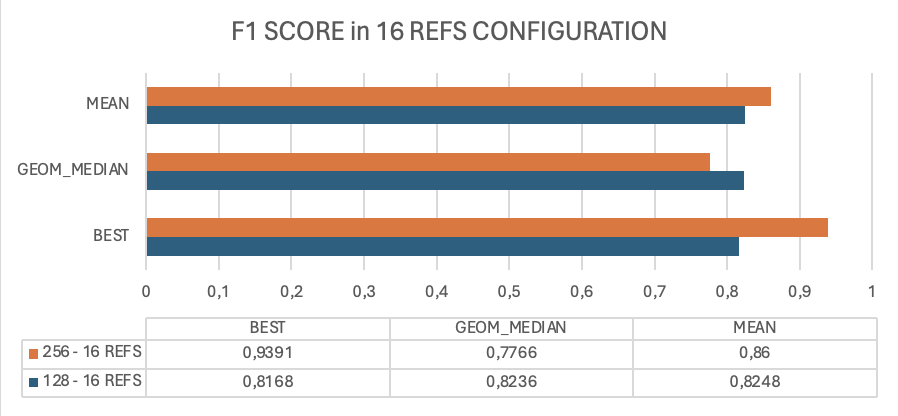
\includegraphics[width=\textwidth]{images/5.03 F1 Score 16 CNN.png}
            \caption{F1 Score with 16 References ($<$EER)}
            \label{fig:f1 score in configurations with 16 refs}
    \end{minipage}
    \hfill
    \begin{minipage}[b]{0.5\textwidth}
            \centering
            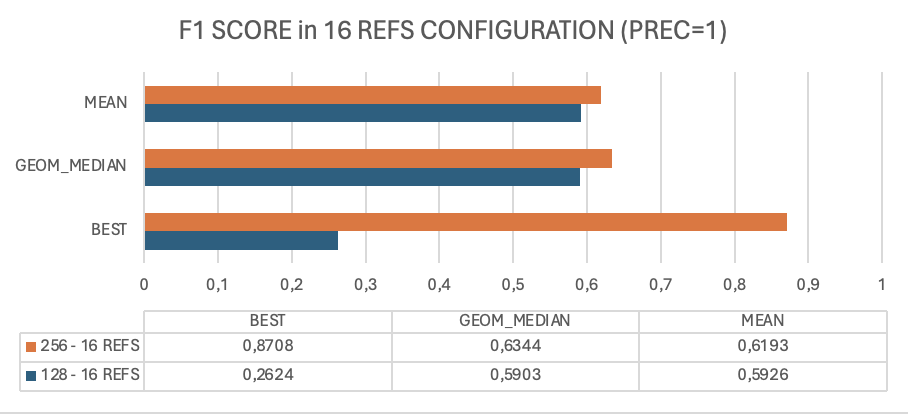
\includegraphics[width=\textwidth]{images/5.04 F1 Score 16 CNN prec1.png}
            \caption{F1 Score with 16 References (PREC=1)}
            \label{fig:f1 score in configurations with 16 refs (prec=1)}
    \end{minipage}
\end{figure}
\subsection{Distillation Knowledge and SV Dense Neural Networks}
\label{sec:distillation knowledge and sv dense neural networks}
The models seen in the previous chapter were Convolutional; however, as introduced before, Syntiant NDP101 doesn't support this type of models, but only Dense Neural Network. Because of this reason, it should be applied the distillation knowledge introduced in \textbf{Subsection \ref{subsec:knowledge distillation training}} to these two convolutional models. The test models with the new create dense configurations consist in the ones introduced in \textbf{Section \ref{sec:test models}}. It is important to remark that the model 256-256 does not fit inside Syntiant NDP101 and it is only taken as reference, because it should be an optimal case that should outperform the other proposed, because of no neuron's reduction and having the most trainable parameters that should mimic better than the others the behavior of the Convolutional Neural Network. 
The training of this Dense Model is performed by parse training input samples to the original model, that will no modify its training parameters, then the student one tries to mimic the output and the training parameters will modify according to the accuracy which will be cosine similarity and the loss 1-cosine similarity, because the objective is to have the two models having the outputs as close as possible. For possible future optimization of the models may be performed a layer per layer aware training, but to verify if the model can work with a standard distillation knowledge it was decided to focus on verify the possible versions deployable instead of optimizing them with more consistent solutions. Averagely, the cosine similarity of the output vectors is around 87,5\%. Distilled every models, the dataset of Speaker Verification was given in input to them. It contains only the samples that passed KWS, Sheila words above 80\% probability, so 2014 samples (453 positives and 1761 negatives). 
\begin{figure}[!h]
    \begin{minipage}[b]{0.5\textwidth}
            \centering
            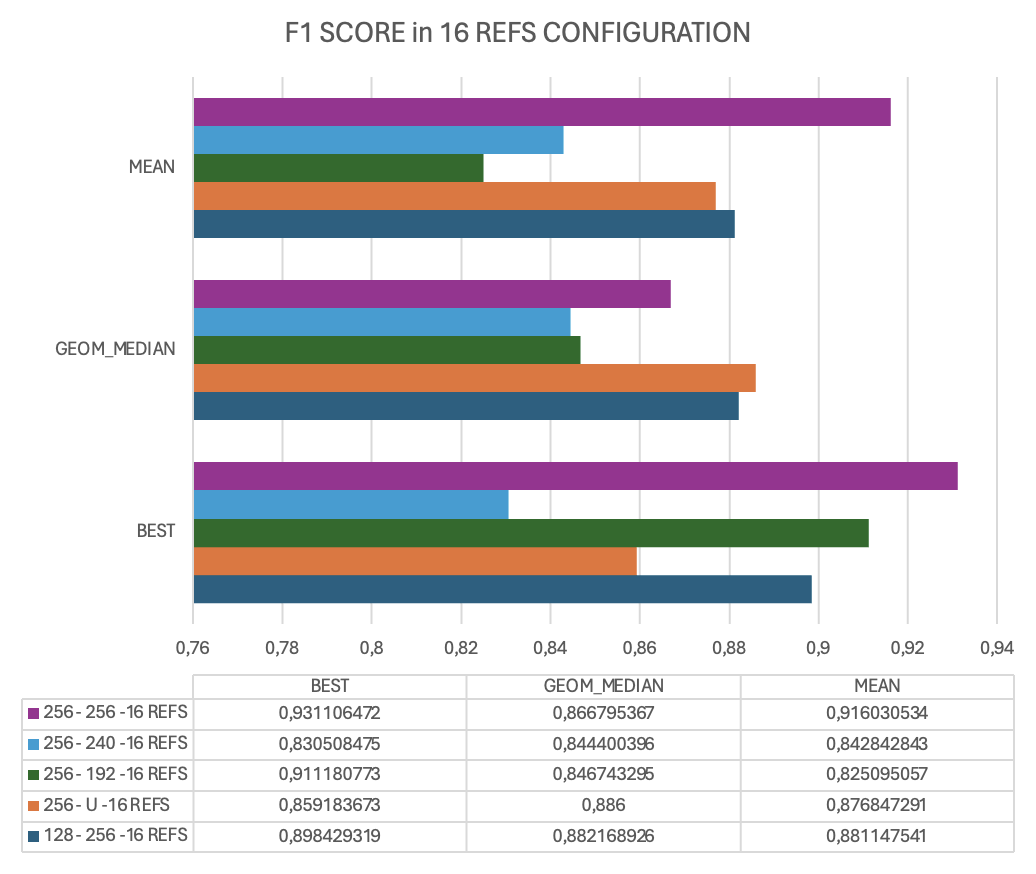
\includegraphics[width=\textwidth]{images/5.05 F1 Score 16 DNN.png}
            \caption{F1 Score with 16 References ($<$EER)}
            \label{fig:f1 score in configurations with 16 refs dnn}
    \end{minipage}
    \hfill
    \begin{minipage}[b]{0.5\textwidth}
            \centering
            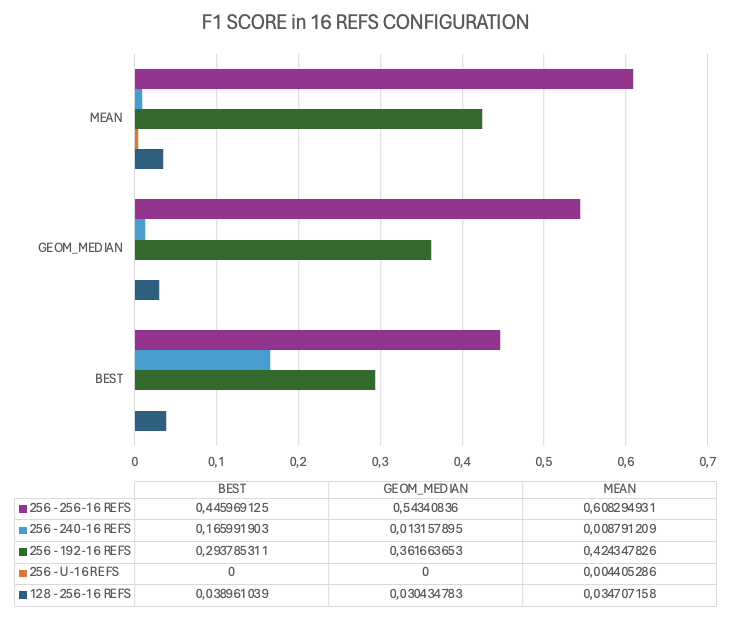
\includegraphics[width=\textwidth]{images/5.06 F1 Score 16 DNN prec1.png}
            \caption{F1 Score with 16 References (PREC=1)}
            \label{fig:f1 score in configurations with 16 refs (prec=1) dnn}
    \end{minipage}
\end{figure}
\newpage
The results obtained by the five models in both minimum EER and precision equal to 1 case, can be seen respectively in \textbf{Table \ref{table:dnnerr}} and in \textbf{Table \ref{table:dnnnofp}}. Starting with minimum EER case, some patterns from Convolutional models are recurring, as fact, single reference give poor performances as are still unsufficient to be a solid structure. Going up with the number the accuracy and F1 Score continue increasing, arriving at 64 references that starts manifesting in some models so inefficiency in recall like saw in Convolutional results. As it is logical the EER performance decreases significantly with more references. According, to the reference perspective the best case should be the 16 references one, which results are displayed in \textbf{Table \ref{fig:f1 score in configurations with 16 refs dnn}}. From that it is seeable that BEST method achieves the best results as expected, GEOM\_MEDIAN gives more stable ones, minimizing the impact of some outliers and generally performs slightly better than MEAN method except in 256-256 case, which is not applicable in this case for Memory Flash space reasons, so overall to save space, even though it is a more energy consumption algorithm is recommended more GEOM\_MEDIAN. However, as said in \textbf{Subsection \ref{subsec:speaker classification of cnn model}}, using EER it is the threshold in which it is minimized maximizing TP and minimizing FP, but it does not guarantee security, so it is required a study on no FP tolerance version, which results are in \textbf{Figure \ref{fig:f1 score in configurations with 16 refs (prec=1) dnn}}.
In this case, happened that there where cases in which the TP were 0, so to avoid not useful data, the threshold was decreased, leading in same cases in having a precision not equal to 1. These cases can be recognized having a missing column in \textbf{Figure \ref{fig:f1 score in configurations with 16 refs (prec=1) dnn}} and having 0 as value in the detailed table under the figure. In this case, in many configurations can be seen an high false negative rate, but there are 2 critical performance degradation. 
The first one is an overfitting case in BEST Method, as fact GEOM\_MEDIAN outperforms it, underlying that at his threshold these distilled models recognize more outliers. It may be good in sort of a way, but at the same time the false negative rates are pretty high and this leads in making a choose between model optimization or choosing a higher number of reference d-vectors. 
Another necessity to make this choose are the models with good results, because the best performing one consists in 256-256 configuration achieving with BEST 45\%, with GEOM\_MEDIAN 54\% and with MEAN 61\%, which are the best ones, but it means the recall is even less (around 50\% in MEAN case) and the model does not fit on Syntiant. 
Increasing the references number to 64 references, are obtained the results in \textbf{Table \ref{fig:f1 score in configurations with 64 refs dnn}} and \textbf{Table \ref{fig:f1 score in configurations with 64 refs (prec=1) dnn}}. In EER minimization case, the results for not optimized or unbalanced versions have slightly worse results, instead in 256-256 which is the most consist one it should perform better, 
but the other are still good results which can be used in a general purpose use scenario. Instead, in no FP tolerance case, the problems of 16 references configurations are resolved, having as expected 256-256 that performs as the best one, having in BEST case over 80\% of F1 Score, indicating a Recall around 70\%, which can be acceptable, however the model does not fit on Syntiant, so if a use have to use a security approach on Syntiant should use 256-192 model, which in BEST case has a F1 score around 58\%, but a recall around 41\% which is not optimal in size terms and in performance, but using these unoptimized models these are the best results obtainable to obtain a precision of 1.
\begin{figure}[!h]
    \begin{minipage}[b]{0.5\textwidth}
            \centering
            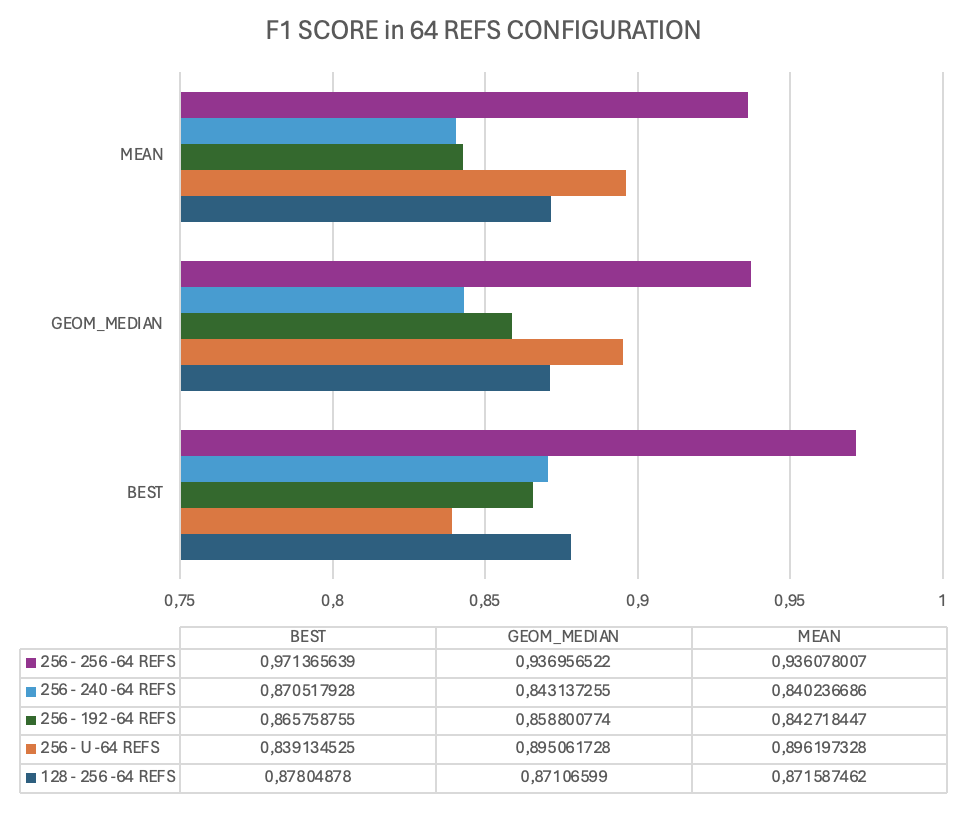
\includegraphics[width=\textwidth]{images/5.07 F1 Score 64 DNN.png}
            \caption{F1 Score with 64 References ($<$EER)}
            \label{fig:f1 score in configurations with 64 refs dnn}
    \end{minipage}
    \hfill
    \begin{minipage}[b]{0.5\textwidth}
            \centering
            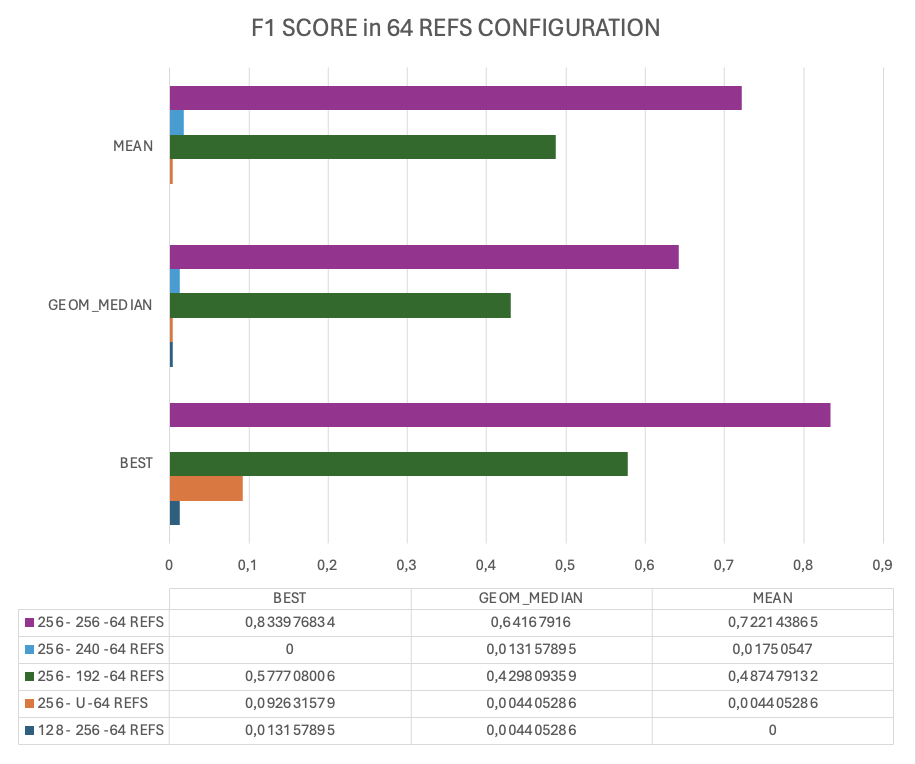
\includegraphics[width=\textwidth]{images/5.08 F1 Score 64 DNN prec1.png}
            \caption{F1 Score with 64 References (PREC=1)}
            \label{fig:f1 score in configurations with 64 refs (prec=1) dnn}
    \end{minipage}
\end{figure}
\newpage
